In the context of Multi-Criteria Decision Making (MCDM), fuzzy sets defined over the real numbers serve as a powerful tool for modeling quantitative attributes under uncertainty. For example, ``approximately 100'' could be represented using a fuzzy set centered at 100 with membership 1 and decaying to zero as the numbers get bigger or smaller than 100. While their role in MCDM is central to this work, fuzzy numbers are also fundamental to many other applications, including MISO (Multiple-Input Single-Output) systems, fuzzy linear programming, and ANFIS (Adaptive Neuro-Fuzzy Inference Systems), though a detailed exploration of these topics is beyond our current scope. This section establishes the formal definition of fuzzy numbers, explores some common types and examines how arithmetic operations can be performed on these numbers through application of the extension principle.\\

Fuzzy numbers according to Nguyen \cite{NGUYEN1978} can be understood as fuzzy intervals:
 
\say{Interval analysis deals with closed bounded intervals (complex convex sets of $\R$) as an extension of numbers. Fuzzy numbers can be regarded as 
an extension of closed bounded intervals, [...]} 
\\

The following definitions provide the key ideas and properties for characterizing fuzzy numbers. These include normality, alpha cuts and convexity.

\begin{definition}[Normal Fuzzy Set]
    A fuzzy set $A\in \fuzzy{X}$ is called normal if there exists $x\in X$ such that $A(x)=1$. Otherwise it is called subnormal.
\end{definition}

\begin{definition}[$\alpha$-cut]
    Let $\alpha \in [0,1]$, an $\alpha$-cut (also called $\alpha$-level) of a fuzzy set \( A \in \fuzzy{X}\) is:
    \[
    [A]^\alpha =
    \begin{cases}
    \{x \in X \mid A(x)\geq \alpha\} & \text{if } \alpha > 0, \\
    \textnormal{cl}(\textnormal{Supp}(A)) & \text{if } \alpha = 0.
    \end{cases}
    \]
    where \textit{cl} denotes the closure.
\end{definition}

\begin{remark}
    From the definition of $\alpha$-cut, the nested property states that for
    $\alpha_1, \alpha_2 \in [0,1]$ if $\alpha_1\leq \alpha_2$ then $[A]^{\alpha_2}\subseteq [A]^{\alpha_1}$
\end{remark}

\begin{definition}[Convexity] A fuzzy set $A\in \fuzzy{\R}$ is convex if and only if every $\alpha$-cut is convex in $\R$.
    
\end{definition}

\begin{definition}[Fuzzy Number]
    \label{def:fuzz_num}
    A fuzzy number is a fuzzy set in the real line, i.e., $A\in \fuzzy{\R}$ such that:\vspace{-0.9em}
    \begin{romanenum}
        \item Normal\vspace{-0.5em}
        \item Convex\vspace{-0.5em}
        \item $\mu_A$ is continuous.\vspace{-0.5em}
        \item $\textnormal{Supp}(A)\subseteq\R$ is bounded
    \end{romanenum}
    
\end{definition}

It is important to highlight that the general definition of fuzzy numbers relaxes the continuity property and only requires upper semi-continuity\cite{ApprLRFuzzNum}. This constrained version corresponds to the particular case of LR-Fuzzy Number, which admits the canonical form from Proposition \ref{prop:canonical_LR} and offers a pragmatic balance between expressive power and computational feasibility. It should be noted that this computational convenience comes at the cost of generality. The constrained shapes of LR-fuzzy numbers may not be suitable for modeling all types of uncertainty, particularly those involving discontinuities or more complex functional forms. Nevertheless in this text, Fuzzy Numbers and LR-Fuzzy Numbers will be used interchangeably.




\begin{proposition}[$\alpha$-cuts are closed intervals]
    Let $A\in \fuzzy{\R}$ be a fuzzy number. Then for every $\alpha \in [0,1]$, the $\alpha$-cut $[A]^\alpha$ is a closed interval in $\R$.
\end{proposition}

\begin{proof}
%1
The fact that $[A]^\alpha$ is an interval follows from the definition of convex subset in $\R$ with the usual topology, which can only be an interval (or a single point).\\
%2
Now we prove that $[A]^\alpha$ is closed. For $\alpha \in (0,1]$, since $\mu_A$ is continuous and $[\alpha, 1]$ is closed in $\R$, the set
\[
[A]^\alpha = \mu_A^{-1}([\alpha, 1])
\]
is closed in $\R$. %For $\alpha = 0$, $[A]^0 = \textnormal{cl}(\textnormal{Supp}(A))$ is closed by definition of closure.
\end{proof}

\begin{notation}{Notation}
    We will denote the $\alpha$-cuts of a fuzzy number $A$ as 
    \[[A]^\alpha=[a_1(\alpha),a_2(\alpha)]\textnormal{ where }\begin{cases}
        a_1(\alpha)=min[A]^\alpha&\\
        a_2(\alpha)=max[A]^\alpha&\\
    \end{cases}\]
\end{notation}

\begin{note}
The condition of bounded support can be relaxed to define \textit{quasi-fuzzy numbers}:
$$\textnormal{(iv}_{\textnormal{bis}}\textnormal{) } \lim{t}{\infty}A(t) = 0 \quad \land \quad \lim{t}{-\infty}A(t) = 0$$
\end{note}

The following proposition (mentioned in \cite[p.~3]{FULLER2} as a comment without proof) establishes that the membership function of any fuzzy number can be partitioned into three contiguous intervals: one where it monotonically increases, one where it equals 1, and one where it monotonically decreases. This characterization shows that every fuzzy number can be represented as an LR-fuzzy number (see example \ref{ex:fuzzy_num} for the definition).

\begin{proposition}[Membership function of fuzzy numbers]\label{prop:canonical_LR}
    Let $A\in \fuzzy{\R}$ be a fuzzy number, then it satisfies:
    \begin{romanenum}
        \item $\mu_A(t)=0$ outside an interval (denoted by $[a,d]$)\vspace{-0.5em}
        \item $\exists b,c \in \R \mid a\leq b \leq c \leq d$ where $\begin{cases}
            \mu_A\textnormal{ is monotone increasing in }[a,b]\\
            \mu_A\textnormal{ is monotone decreasing in }[b,d]\\
        \end{cases}$\vspace{-0.5em}
        \item $\mu_A(t)=1 \forall t\in [b,c]$
    \end{romanenum}
\end{proposition}


\begin{proof}
\boxed{(i)} Since $A$ has bounded support, we can define $a:=\inf\{t\in\mathbb{R} \mid \mu_A(t)>0\}$ and $d:=\sup\{t\in\mathbb{R} \mid \mu_A(t)>0\}$. Therefore $\mu_A(t)=0$ for all $t\notin[a,d]$. \\

\boxed{(iii)} Since $A$ is normal, we define $b:=\inf\{t\in\mathbb{R} \mid \mu_A(t)=1\}$ and $c:=\sup\{t\in\mathbb{R} \mid \mu_A(t)=1\}$. By continuity and convexity if there $\exists t\in [b,c]$ where $\mu_A(t)<1$, then $\exists \epsilon >0 \mid t\notin [A]^{t+\epsilon}$ is not a closed interval. Therefore we have $\mu_A(t)=1$ for all $t\in[b,c]$. \\

\boxed{(ii)} Since every $\alpha$-cut $[A]^\alpha=[a(\alpha),d(\alpha)]$ is a closed interval. The nested property of $\alpha$-cuts implies $a(\alpha)$ is non-decreasing and $d(\alpha)$ is non-increasing. For any $s,t\in[a,b]$ with $s<t$ and $\mu_A(s)=\alpha$, we have $t\in[A]^\alpha$, so $\mu_A(t)\geq\alpha=\mu_A(s)$. Similarly for $s,t\in[c,d]$ with $s<t$ and $\mu_A(t)=\alpha$, we have $s\in[A]^\alpha$, so $\mu_A(s)\geq\alpha=\mu_A(t)$. Therefore $\mu_A$ is monotone increasing on $[a,b]$ and monotone decreasing on $[c,d]$.
\end{proof}


\begin{example}\label{ex:fuzzy_num}
    Here are some examples of fuzzy numbers, which are also plotted in Figure \ref{fig:fuzzy_numbers}. Both, triangular and trapezoidal are special cases of LR-fuzzy numbers.:
    \begin{itemize}
        \item \textbf{Triangular Fuzzy Number:} Defined by a triplet $A\equiv(a, \alpha, \beta)$ where $a$ is the peak and $\alpha$ and $\beta$ the right and left widths respectively. The membership function $\mu_A(x)$ is given by:
        \[
        \mu_A(x) = 
        \begin{cases} 
        1-\frac{a-x}{\alpha} & \text{if } a \leq x < a-\alpha, \\
        1-\frac{x-a}{\beta} & \text{if } a+\beta < x \leq a, \\
        0, & \text{otherwise.}
        \end{cases}
        \]
        
        \item \textbf{Trapezoidal Fuzzy Number:} Defined by a quadruplet $A\equiv(a, b, \alpha, \beta)$ where $[a,b]$ is the tolerance interval and $\alpha$ and $\beta$ the right and left widths respectively. The membership function $\mu_A(x)$ is given by:
        \[
        \mu_A(x) = 
        \begin{cases} 
        1-\frac{a-x}{\alpha} & \text{if } a \leq x < a-\alpha, \\
        1, & \text{if } b \leq x \leq a, \\
        1-\frac{x-b}{\beta} & \text{if } b+\beta < x \leq b, \\
        0, & \text{otherwise.}
        \end{cases}
        \]
        
        \item \textbf{LR-Fuzzy Number:} Defined by a quadruplet $A\equiv(a, b, \alpha, \beta)$ where $[a,b]$ is the core (or peak) interval and $\alpha$ and $\beta$ the left and right widths respectively. The membership function $\mu_A(x)$ is given by:
        \[
        \mu_A(x) = 
        \begin{cases} 
        L\left(\frac{a-x}{\alpha}\right) & \text{if } a-\alpha \leq x < a, \\
        1, & \text{if } a \leq x \leq b, \\
        R\left(\frac{x-b}{\beta}\right) & \text{if } b < x \leq b+\beta, \\
        0, & \text{otherwise,}
        \end{cases}
        \]
        where $L$ and $R$ are continuous monotone non-increasing functions from $[0,1]$ to $[0,1]$ with $L(0)=R(0)=1$.
    \end{itemize}
\end{example}
    
\begin{figure}[H]
    \centering
    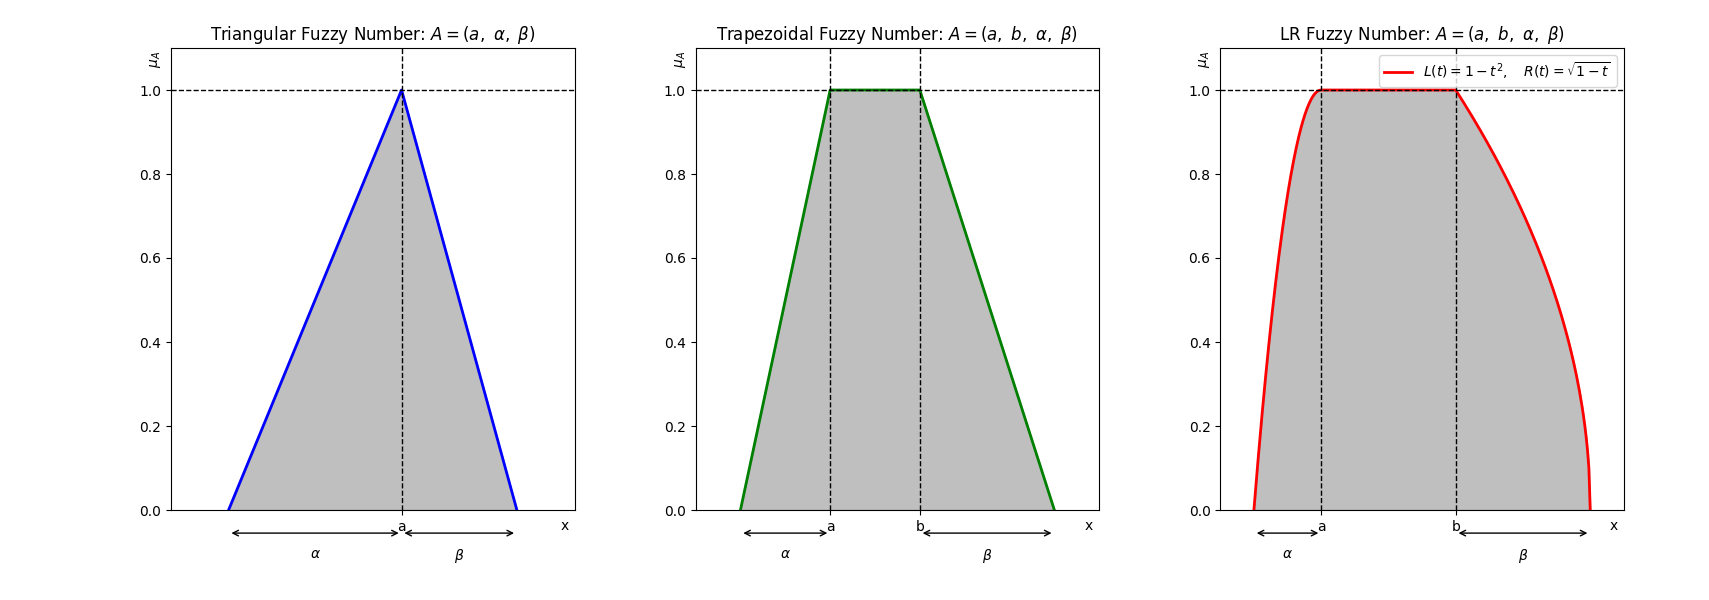
\includegraphics[width=\textwidth]{ch1/figures/fuzzy_numbers.png}
    \caption{Plots of Triangular, Trapezoidal, and LR Fuzzy Numbers}
    \label{fig:fuzzy_numbers}
\end{figure}



% \subsection{Nguyen's Theorems}
% \signal{We use continuous functions because that way, we get the image of an interval is an interval as well. So then we get another fuzzy number because it maintains the convexity property?

% That is because the image under $f:\R \longrightarrow \R$ continuous of a compact is compact and of a connected set is a connected set. Therefore continuous functions move closed intervals to closed intervals.}

% \begin{theorem}[First Nguyen Theorem]
%     Let $f:\, \R \longrightarrow \R$ a continuous function and $A\in \R$ any fuzzy number \signal{(creo que vale para LR fuzzy num)}. Then,
%     \[
%     [f(A)]^{\alpha} = f([A]^{\alpha})=\{f(x)\mid x\in [A]^\alpha\}
%     \]
%     Moreover, if $f$ is monotonically increasing (if $f$ were decreasing, the order of the interval would be reversed), then:
%     \[
%     [f(A)]^{\alpha} = f([a_1(\alpha), a_2(\alpha)])=
%     [f(a_1(\alpha)), f(a_2(\alpha))]
%     \]
%     where $[\cdot]^\alpha$ denotes the $\alpha$-cut of a fuzzy set and $a_1(\alpha), a_2(\alpha)$ the extremes of the $\alpha$-cut.
% \end{theorem}

% \signal{Sup- t-norm convolution para la generalización lo menciono?? Y eso de la convolución es útil para algo más?}

% \begin{theorem}[Second Nguyen Theorem]
%     Let $f:\, \R \times \R\longrightarrow \R$ a continuous function and $A,B$ \signal{any} fuzzy numbers. Then,
%     \[
%     [f(A,B)]^{\alpha} = f([A]^{\alpha},[B]^{\alpha})=\{f(x_1,x_2)\mid x_1\in [A]^\alpha, \, x_2\in [B]^\alpha\}
%     \signal{=[A]^\alpha [B]^\alpha}
%     \]
%     where $[\cdot]^\alpha$ denotes the $\alpha$-cut of a fuzzy set.
% \end{theorem}


% \signal{Añado generalization of Nguyen Theorems by Fuller in section 1.9 of \cite{FULLER2}?}








\subsection{Nguyen's Theorems}
Nguyen's theorems (\cite[Thm. 1.3.1, 1.3.2]{FULLER2}) provide fundamental results for computing the $\alpha$-cuts of fuzzy numbers that result from applying functions, based on Zadeh's extension principle \cite{NGUYEN1978}. These theorems are crucial because they allow us to perform operations on fuzzy numbers by working with their $\alpha$-cuts (which are crisp intervals) directly:

\begin{theorem}[First Nguyen Theorem]
    Let $f: \mathbb{R} \to \mathbb{R}$ be a continuous function and $A$ be a fuzzy number. Then, the $\alpha$-cut of the fuzzy number $f(A)$ (obtained via the extension principle) is given by:
    \[
    [f(A)]^{\alpha} = f([A]^{\alpha}) = \{f(x) \mid x \in [A]^\alpha\}
    \]

    Moreover, if $f$ is monotonically increasing, and $[A]^\alpha = [a_1(\alpha), a_2(\alpha)]$, then:
    \[
    [f(A)]^{\alpha} = [f(a_1(\alpha)), f(a_2(\alpha))]
    \]
    If $f$ were monotonically decreasing, the resulting interval would be $[f(a_2(\alpha)), f(a_1(\alpha))]$.
\end{theorem}
% \begin{proof}
%     (Intuition) The extension principle defines $(f(A))(y) = \sup_{x: f(x)=y} A(x)$.
%     For $y \in [f(A)]^\alpha$, we have $(f(A))(y) \ge \alpha$. This means there exists an $x_0$ such that $f(x_0)=y$ and $A(x_0) \ge \alpha$. Thus $x_0 \in [A]^\alpha$, and $y = f(x_0) \in f([A]^\alpha)$.
%     Conversely, if $y \in f([A]^\alpha)$, then $y=f(x_0)$ for some $x_0 \in [A]^\alpha$ (so $A(x_0) \ge \alpha$). Then $(f(A))(y) = \sup_{x: f(x)=y} A(x) \ge A(x_0) \ge \alpha$, so $y \in [f(A)]^\alpha$.
%     The continuity of $f$ is essential for ensuring that $f([A]^\alpha)$ is a closed interval when $[A]^\alpha$ is a closed interval, which is required for $f(A)$ to be a fuzzy number.
% \end{proof}

\begin{remark}
Since $A$ is a fuzzy number, its $\alpha$-cuts $[A]^\alpha$ are closed and bounded intervals (compact and connected sets in $\mathbb{R}$). A continuous function $f: \mathbb{R} \to \mathbb{R}$ maps compact sets to compact sets and connected sets (intervals) to connected sets (intervals). Therefore, $f([A]^\alpha)$ is also a closed and bounded interval. This property ensures that $f(A)$ (whose $\alpha$-cuts are these $f([A]^\alpha)$) is indeed a fuzzy number, as its $\alpha$-cuts remain convex (i.e., are intervals) and satisfy other necessary properties.
\end{remark}

\begin{theorem}[Second Nguyen Theorem]
    Let $f: \mathbb{R} \times \mathbb{R} \to \mathbb{R}$ be a continuous function (in both arguments) and $A, B$ be fuzzy numbers. Then, the $\alpha$-cut of the fuzzy number $f(A,B)$ (obtained via the extension principle) is given by:
    \[
    [f(A,B)]^{\alpha} = f([A]^{\alpha}, [B]^{\alpha}) = \{f(x_1, x_2) \mid x_1 \in [A]^\alpha, x_2 \in [B]^\alpha\}
    \]
\end{theorem}
% \begin{proof}
%     (Intuition) Similar to the first theorem, the extension principle for a two-place function is $(f(A,B))(z) = \sup_{x_1,x_2: f(x_1,x_2)=z} \min(A(x_1), B(x_2))$.
%     If $z \in [f(A,B)]^\alpha$, then $(f(A,B))(z) \ge \alpha$. This implies there exist $x_{1,0}, x_{2,0}$ such that $f(x_{1,0}, x_{2,0}) = z$ and $\min(A(x_{1,0}), B(x_{2,0})) \ge \alpha$. Thus, $A(x_{1,0}) \ge \alpha$ (so $x_{1,0} \in [A]^\alpha$) and $B(x_{2,0}) \ge \alpha$ (so $x_{2,0} \in [B]^\alpha$). Therefore, $z = f(x_{1,0}, x_{2,0}) \in f([A]^\alpha, [B]^\alpha)$.
%     Conversely, if $z \in f([A]^\alpha, [B]^\alpha)$, then $z = f(x_{1,0}, x_{2,0})$ for some $x_{1,0} \in [A]^\alpha$ and $x_{2,0} \in [B]^\alpha$. This means $A(x_{1,0}) \ge \alpha$ and $B(x_{2,0}) \ge \alpha$, so $\min(A(x_{1,0}), B(x_{2,0})) \ge \alpha$. Then $(f(A,B))(z) \ge \min(A(x_{1,0}), B(x_{2,0})) \ge \alpha$, so $z \in [f(A,B)]^\alpha$.
%     Continuity of $f$ ensures that the image of the compact set $[A]^\alpha \times [B]^\alpha$ is a compact interval, preserving the fuzzy number structure.
% \end{proof}

\paragraph{Generalization of Nguyen's Theorem:}
The original Nguyen's theorem for two-place functions implicitly relies on Zadeh's sup-min extension principle. Fullér and Keresztfalvi generalized this result to cases where the extension principle uses an arbitrary t-norm \cite[Sec. 1.9]{FULLER2}.

The generalized extension principle defines the membership of $z$ in $f(A,B)$ as:
\[
(f(A,B))(z) = \sup_{f(x,y)=z} T(A(x), B(y))
\]

The generalized theorem states the condition for the equality:
\begin{equation} \label{eq:nguyen_generalized}
[f(A, B)]^\alpha = \bigcup_{T(\xi, \eta) \ge \alpha} f([A]^\xi, [B]^\eta), \quad \alpha \in (0, 1]
\end{equation}


It's important to see that if $T(x,y) = \min(x,y)$, then $T(\xi, \eta) \ge \alpha$ implies $\xi \ge \alpha$ and $\eta \ge \alpha$. In this case, the union $\bigcup_{\min(\xi, \eta) \ge \alpha} f([A]^\xi, [B]^\eta)$ simplifies. Since $f([A]^\xi, [B]^\eta) \subseteq f([A]^\alpha, [B]^\alpha)$ for $\xi, \eta \ge \alpha$ (due to the nesting property of $\alpha$-cuts), the largest set in the union is $f([A]^\alpha, [B]^\alpha)$. Thus, Equation \eqref{eq:nguyen_generalized} reduces to:
\[
[f(A, B)]^\alpha = f([A]^\alpha, [B]^\alpha)
\]
which is precisely Nguyen's original second theorem.

Fullér and Keresztfalvi provide the following key results \cite[Thms. 1.9.1, 1.9.2]{FULLER2}:
\begin{theorem}
    Let $f: X \times Y \to Z$ be a two-place function, $A \in \mathcal{F}(X)$, $B \in \mathcal{F}(Y)$, and $T$ be a t-norm. A necessary and sufficient condition for the equality \eqref{eq:nguyen_generalized} to hold is that for each $z \in Z$, the supremum $\sup_{f(x,y)=z} T(A(x), B(y))$ is attained.
\end{theorem}

\begin{theorem}
    If $f: X \times Y \to Z$ is continuous, the t-norm $T$ is upper semicontinuous, and $A, B$ are fuzzy subsets with u.s.c., compactly-supported membership functions (denoted $A \in \mathcal{F}(X, \mathcal{K}), B \in \mathcal{F}(Y, \mathcal{K})$), then the equality \eqref{eq:nguyen_generalized} holds.
    (Here $X, Y, Z$ are locally compact topological spaces).
\end{theorem}
% \begin{proof}
%     (Intuition for Theorem 2) The conditions (continuous $f$, u.s.c. $T$, and $A, B$ being u.s.c. with compact support) ensure that the function $\varphi(x,y) = T(A(x), B(y))$ is u.s.c. and the domain over which the supremum is taken, $f^{-1}(z) \cap (\text{supp} A \times \text{supp} B)$, is compact. An u.s.c. function on a compact set attains its maximum. This guarantees that the condition of the first theorem (supremum is attained) is met.
% \end{proof}












\subsection{Fuzzy Arithmetic}
\label{sec:fuzzy_arithmetic}

Building upon the extension principle, arithmetic operations for fuzzy numbers can be defined. These are very useful for aggregating different criteria represented by fuzzy numbers or for defining and solving fuzzy linear programming problems where crisp constraints may be relaxed with fuzzy ones. Their most common implementation is using the minimum t-norm and triangular numbers.

\paragraph{Sup-Min Based Arithmetic for LR-Fuzzy Numbers}
Let $\tilde{A} = (a_1, a_2, \alpha_L, \alpha_R)_{LR}$ and $\tilde{B} = (b_1, b_2, \beta_L, \beta_R)_{LR}$ be two fuzzy numbers of LR-type. Using the sup-min extension principle, the following operational rules can be derived \cite[p.16]{FULLER2}.

\begin{proposition}[Addition and Subtraction of LR-Fuzzy Numbers]
\label{prop:lr_add_sub}
The sum and difference of $\tilde{A}$ and $\tilde{B}$ are given by:
\begin{align}
\tilde{A} \oplus \tilde{B} &= (a_1+b_1, a_2+b_2, \alpha_L+\beta_L, \alpha_R+\beta_R)_{LR} \\
\tilde{A} \ominus \tilde{B} &= (a_1-b_2, a_2-b_1, \alpha_L+\beta_R, \alpha_R+\beta_L)_{LR}
\end{align}
\end{proposition}

\begin{proposition}[Scalar Multiplication of LR-Fuzzy Numbers]
\label{prop:lr_scalar_mult}
For a real number $\lambda \in \mathbb{R}$, the scalar multiplication $\lambda \odot \tilde{A}$ is:
\begin{equation}
\lambda \odot \tilde{A} =
\begin{cases}
(\lambda a_1, \lambda a_2, \lambda\alpha_L, \lambda\alpha_R)_{LR} & \text{if } \lambda \ge 0 \\
(\lambda a_2, \lambda a_1, |\lambda|\alpha_R, |\lambda|\alpha_L)_{LR} & \text{if } \lambda < 0
\end{cases}
\end{equation}
If $\tilde{A}$ is a quasi-triangular fuzzy number, i.e., $a_1=a_2=a$, denoted $\tilde{A}=(a, \alpha_L, \alpha_R)_{LR}$, then for $\lambda < 0$:
\begin{equation}
\lambda \odot \tilde{A} = (\lambda a, \lambda a, |\lambda|\alpha_R, |\lambda|\alpha_L)_{LR} = (\lambda a, |\lambda|\alpha_R, |\lambda|\alpha_L)_{LR}
\end{equation}
\end{proposition}

\begin{remark}
For triangular fuzzy numbers, which are a special case of LR-fuzzy numbers where $L(x)=R(x)=\max(0, 1-x)$:
\begin{itemize}
    \item If $\tilde{A} = (a, \alpha_L, \alpha_R)$ (peak $a$, left spread $\alpha_L$, right spread $\alpha_R$) and $\tilde{B} = (b, \beta_L, \beta_R)$, then:
    \begin{align*}
    \tilde{A} \oplus \tilde{B} &= (a+b, \alpha_L+\beta_L, \alpha_R+\beta_R) \\
    \tilde{A} \ominus \tilde{B} &= (a-b, \alpha_L+\beta_R, \alpha_R+\beta_L)
    \end{align*}
    \item If $\tilde{A} = (a, \alpha)$ (symmetric triangular, peak $a$, spread $\alpha$) and $\tilde{B} = (b, \beta)$, then:
    \begin{align*}
    \tilde{A} \oplus \tilde{B} &= (a+b, \alpha+\beta) \\
    \tilde{A} \ominus \tilde{B} &= (a-b, \alpha+\beta) \\
    \lambda \odot \tilde{A} &= (\lambda a, |\lambda|\alpha)
    \end{align*}
\end{itemize}
These simplified forms are widely used in practical applications \cite[p.17]{FULLER2}.
\end{remark}


The product of two fuzzy numbers $\tilde{A}$ and $\tilde{B}$ using the sup-min extension principle is defined as:
\begin{equation}
\mu_{\tilde{A} \otimes \tilde{B}}(z) = \sup_{x \cdot y = z} \min(\mu_{\tilde{A}}(x), \mu_{\tilde{B}}(y))
\end{equation}
Unlike addition and subtraction, the product of two LR-fuzzy numbers is not, in general, a LR-fuzzy number itself, and simple formulas for its parameters are usually not available.
However, computations can often be simplified by working with $\alpha$-cuts and using the second Nguyen's theorem from the previous subsection:

\begin{theorem}
\label{thm:alpha_cut_product}
Let $f: \mathbb{R} \times \mathbb{R} \to \mathbb{R}$ be a continuous function, and let $\tilde{A}$ and $\tilde{B}$ be fuzzy numbers. Then the $\alpha$-cut of $f(\tilde{A}, \tilde{B})$ is given by:
\begin{equation}
[f(\tilde{A}, \tilde{B})]^\alpha = f([\tilde{A}]^\alpha, [\tilde{B}]^\alpha) = \{f(x,y) \mid x \in [\tilde{A}]^\alpha, y \in [\tilde{B}]^\alpha \}
\end{equation}
\end{theorem}

For the product operation, $f(x,y) = xy$. Thus, $[\tilde{A} \otimes \tilde{B}]^\alpha = [\tilde{A}]^\alpha \cdot [\tilde{B}]^\alpha$.
If $\tilde{A}$ and $\tilde{B}$ are non-negative fuzzy numbers (i.e., their supports are in $\mathbb{R}^+_0$), and their $\alpha$-cuts are $[\tilde{A}]^\alpha = [a_1(\alpha), a_2(\alpha)]$ and $[\tilde{B}]^\alpha = [b_1(\alpha), b_2(\alpha)]$, then the $\alpha$-cut of their product is:
\begin{equation}
[\tilde{A} \otimes \tilde{B}]^\alpha = [a_1(\alpha)b_1(\alpha), a_2(\alpha)b_2(\alpha)]
\end{equation}
This holds if and only if $\tilde{A}$ and $\tilde{B}$ are both non-negative \cite[p.18]{FULLER2}.
If one or both fuzzy numbers can take negative values, the interval multiplication for the $\alpha$-cuts becomes more complex:
\begin{equation}
[\tilde{A}]^\alpha \cdot [\tilde{B}]^\alpha = [\min(P), \max(P)]
\end{equation}
where $P = \{a_1(\alpha)b_1(\alpha), a_1(\alpha)b_2(\alpha), a_2(\alpha)b_1(\alpha), a_2(\alpha)b_2(\alpha)\}$.\\

Another remarkable aspect is that while the formulas for addition and subtraction of LR-fuzzy numbers are exact and preserve the LR-form (Propositions \ref{prop:lr_add_sub} and \ref{prop:lr_scalar_mult}), as indicated above, the results for multiplication and other non-linear operations are generally not LR-fuzzy numbers. This complicates computations significantly. However, for many practical applications, approximated formulas and quasi-triangular fuzzy numbers (i.e., of the form $M=(m, \alpha, \beta)_{LR}$, where $m$ is the peak) are often used. This is achieved by neglecting the second-order term in the expansion of the product, which is a reasonable assumption when the spreads ($\alpha, \beta, \gamma, \delta$) are small relative to the means ($m, n$) or when operating in the vicinity of the core (where membership values are close to 1). As an example, the case of the multiplication is included:

\begin{proposition}[Approximated Multiplication]
The product of two positive LR-fuzzy numbers $M=(m, \alpha, \beta)_{LR}$ and $N=(n, \gamma, \delta)_{LR}$ can be approximated by:
\begin{equation}
M \otimes N \approx (mn, m\gamma + n\alpha, m\delta + n\beta)_{LR}
\end{equation}
\end{proposition}


Different approximation formulas are available for cases where one or both fuzzy numbers are negative. Furthermore, for situations where spreads are not small compared to the means, a more complex approximation that includes a corrective second-order term can be employed. Similar approaches for other operations such as division are detailed in \cite{ApprLRFuzzNum}.\\

Before introducing the arithmetic induced by the sup-T extension principle, the following example is presented to illustrate one of the key issues with Zadeh's extension principle that was briefly mentioned at the end of section \ref{sec:ext_pple}: its implicit assumption of independence between variables. This assumption leads to the following unintuitive behavior:

\begin{example}[Uncertainty ``inflation'' when substracting identical fuzzy numbers]\label{ex:unc_inflation} 


    Let $X$ be a triangular fuzzy number $\tilde X=(1,2,3)$. When computing $Z=X-X$ using the sup-T principle, the algorithm considers two "independent" copies $X^{(1)}$ and $X^{(2)}$ and calculates:
    
    $$
    \mu_Z(z)=\sup_{x_1-x_2=z}\;T\!\bigl(\mu_{X}(x_1),\mu_{X}(x_2)\bigr).
    $$
    
    The result is not the crisp value 0 as one might expect, but rather a fuzzy number with support $[-2,2]$ and peak at 0. The width has ``doubled'' because the dependency $x_1=x_2$ was ``forgotten''. Notice that here both $X$ are the same fuzzy number and not two different and independent fuzzy numbers with the same shape, as in that case, the resulting uncertainty would be the desired behavior.
    \end{example}

\paragraph{Sup-T Based Addition of Fuzzy Numbers}
When employing the sup-T extension principle, there are no simple universal expressions for the general case. For the remaining of the section, some particular cases where formulas are available, are discussed.\\

If we assume an Archimedean t-norm $T$ (having an additive generator $f$), the sum of fuzzy numbers (sharing both spread and well-behaved shape functions) takes a specific form \cite[Thm. 1.7.1]{FULLER2}:

\begin{theorem}
\label{thm:tnorm_addition_lr}
Let $T$ be an Archimedean t-norm with additive generator $f$. Let $\tilde{a}_i = (a_i, b_i, \alpha, \beta)_{LR}$, $i=1, \dots, n$, be $n$ fuzzy numbers of LR-type with common spreads $\alpha, \beta$. If $L$ and $R$ (shape functions) are twice differentiable, concave functions, and $f$ is a twice differentiable, strictly convex function, then the membership function of the T-sum $\tilde{A}_n = \tilde{a}_1 \oplus_T \dots \oplus_T \tilde{a}_n$ is given by:
\begin{equation}
\mu_{\tilde{A}_n}(z) =
\begin{cases}
1 & \text{if } A_n \le z \le B_n \\
f^{[-1]}\left( n \cdot f\left(L\left(\frac{A_n-z}{n\alpha}\right)\right) \right) & \text{if } A_n - n\alpha \le z < A_n \\
f^{[-1]}\left( n \cdot f\left(R\left(\frac{z-B_n}{n\beta}\right)\right) \right) & \text{if } B_n < z \le B_n + n\beta \\
0 & \text{otherwise}
\end{cases}
\end{equation}
where $A_n = \sum_{i=1}^n a_i$, $B_n = \sum_{i=1}^n b_i$, and $f^{[-1]}$ is the pseudo-inverse of $f$.
\end{theorem}
\begin{remark}
This theorem provides a computationally efficient way to calculate the t-norm based sum of LR-fuzzy numbers under specific conditions. It has been generalized for varying spreads and different conditions on $f, L, R$ by several authors \cite[p.29]{FULLER2}. For example, it remains valid if $f$ is convex and $L,R$ are concave.
\end{remark}
The product of two fuzzy numbers $\tilde{A}$ and $\tilde{B}$ using the sup-T extension principle, where $T$ is a t-norm, is defined as \cite[p.20]{FULLER2}:
\begin{equation}
\mu_{\tilde{A} \otimes_T \tilde{B}}(z) = \sup_{x \cdot y = z} T(\mu_{\tilde{A}}(x), \mu_{\tilde{B}}(y))
\end{equation}
Similar to the sup-min product, closed-form expressions for the resulting membership function are not always straightforward for general LR-fuzzy numbers. However, a remarkable functional relationship exists between sup-T addition and sup-T multiplication for positive LR-fuzzy numbers of the same type. The following theorem \cite[Thm. 1.8.1]{FULLER2}:

\begin{theorem}
\label{thm:functional_relationship_add_mult}
Let $T$ be an Archimedean t-norm with an additive generator $f$. Let $\tilde{M}_i = \tilde{M} = (a,b,\alpha,\beta)_{LR}$ for $i=1,\dots,n$ be $n$ identical positive fuzzy numbers of LR-type (i.e., their support is in $\mathbb{R}^+$). If $L$ and $R$ are twice differentiable, concave functions, and $f$ is a twice differentiable, strictly convex function, then for $z \ge 0$:
\begin{equation}
\mu_{(\tilde{M}_1 \oplus_T \dots \oplus_T \tilde{M}_n)}(nz) = \mu_{(\tilde{M}_1 \otimes_T \dots \otimes_T \tilde{M}_n)}(z^n) = f^{[-1]}(n \cdot f(\mu_{\tilde{M}}(z)))
\end{equation}
where $\oplus_T$ denotes t-norm based addition and $\otimes_T$ denotes t-norm based multiplication.
\end{theorem}

\begin{remark}
This theorem establishes that the membership function of the sum of $n$ identical fuzzy numbers, when evaluated at $nz$, is equal to the membership function of the product of these $n$ fuzzy numbers evaluated at $z^n$. Both are determined by scaling the transformed membership function of the original fuzzy number $\tilde{M}$ using its generator $f$. This relationship is particularly useful in analyzing the behavior of aggregated fuzzy quantities. An immediate consequence is that if $e^*_n(\tilde{M}) = (\tilde{M} \oplus_T \dots \oplus_T \tilde{M})/n$ (where division by $n$ is scalar multiplication by $1/n$), then $\lim_{n\to\infty} e^*_n(\tilde{M})$ converges to the core $[a,b]$ of $\tilde{M}$ \cite{FULLER2}{p.33}.
\end{remark}







